\enteteExam{NFE106 -- Administration de bases de données}%
{Examen 14 juin 2024 -- session 1 -- 3h}%
{Examen en présentiel -- Calculatrices autorisées -- Documents autorisés: 5 pages recto/verso de notes personnelles}%

\section{Stockage et indexation (7 pts)}

  \begin{figure}[htb]  
   \centerline{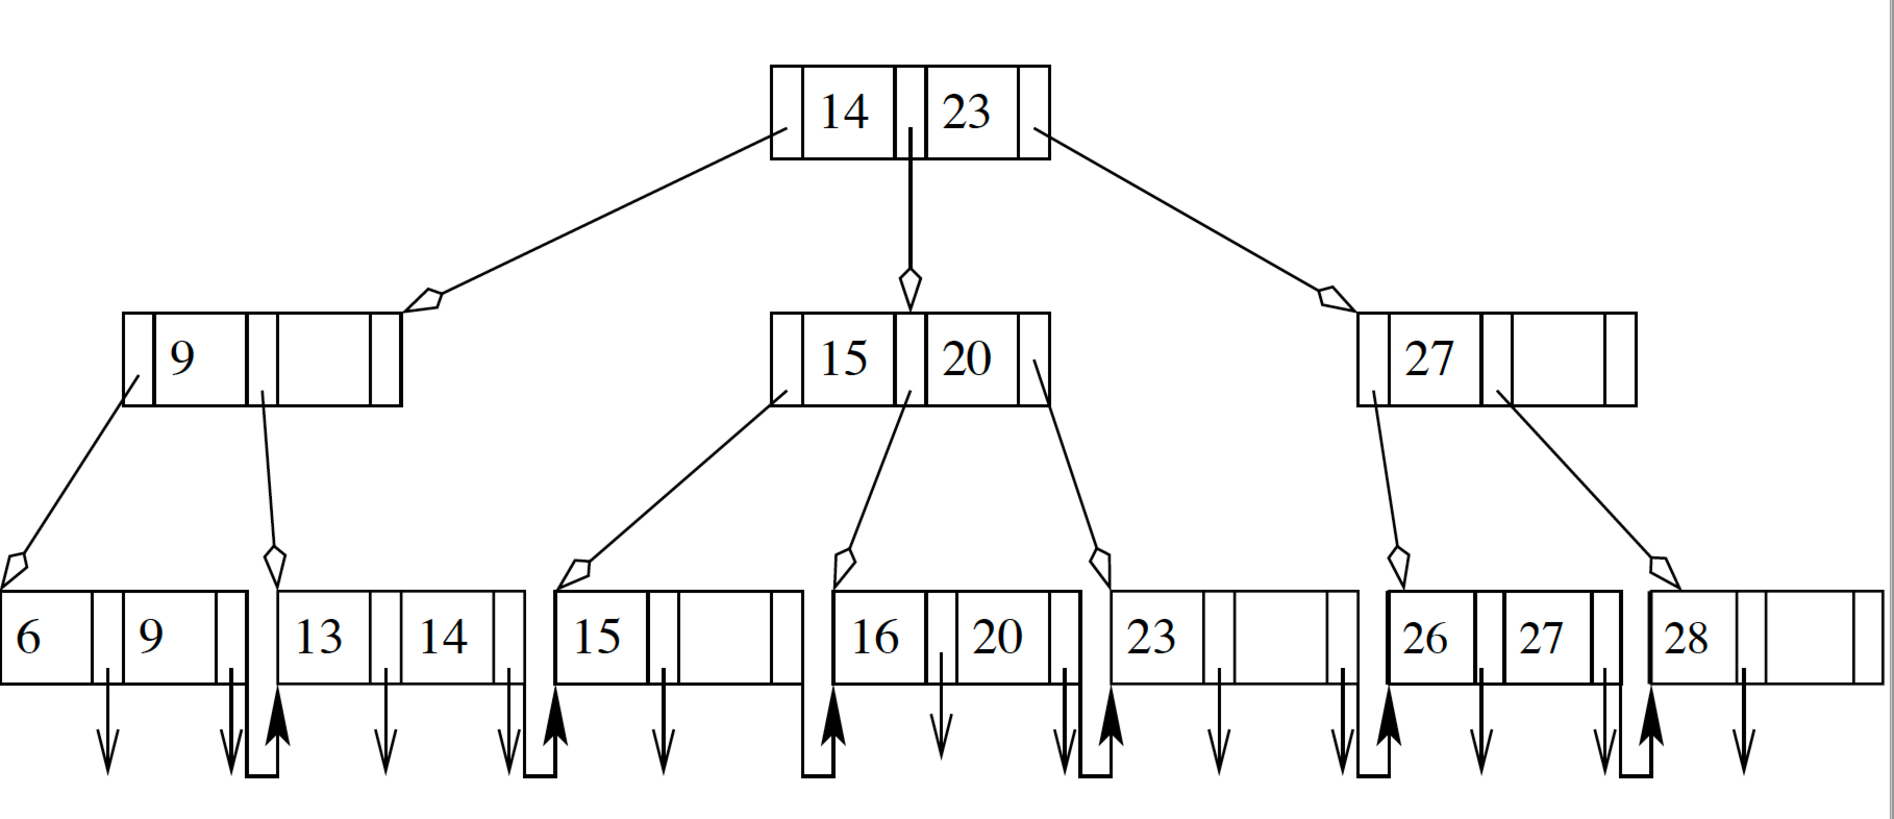
\includegraphics[scale=0.4]{../supports/figures/ex106-s1-hybride-20}}
    \caption{Un arbre B}  
    \label{arbreb}  
  \end{figure} 

\begin{enumerate}
  
  \item Une table relationnelle contient 256\,500 lignes. 
   On la stocke dans une base avec des blocs
de 4\,000 octets. On 
suppose que chaque enregistrement a une taille de 
200 octets et que chaque bloc a un entête de 100 octets. 
Quel est le nombre d'enregistrements par bloc\,? Quel est le
  nombre de blocs nécessaire pour stocker la table
(on suppose que les blocs contiennent autant d'enregistrements
que possible)\,?


\begin{solution}
On place  $\lfloor \frac{3900}{200} \rfloor = 19$ enregistrements par bloc.  Il faut 
        $\lceil \frac{256\,500}{19} \rceil = 13\,500$ blocs.
\end{solution}

  \item La figure~\ref{arbreb} montre un arbre B. On peut stocker au plus 2 entrées par bloc.
         Indiquez le rôle
    des différents pointeurs représentés,

\begin{solution}
 Structure d'un arbre B+: voir le cours.
\end{solution}

 \item Donnez l'arbre après
   insertion d'un enregistrement de clé 17 (dessinez au moins les parties
    de l'arbre qui ont changé).
    
\begin{solution}
L'insertion d'une clé 17 
 entraîne l'éclatement du nœud (16,20) en deux nœuds, 
 (16,17) d'un côté, (20) de l'autre. La valeur médiane (17 donc)
 étant insérée dans le parent (15,20), ce qui entraîne un
 nouvel éclatement. La valeur 17 monte dans la racine, provoque
 un troisième éclatement avec ajout d'un niveau. 17 devient
 donc la valeur de la nouvelle racine de l'arbre.
\end{solution}

  \item On effectue une recherche sur l'intervalle [13,23] (avant l'insertion
  de la clé 17). Combien
  de blocs lit-on dans l'index, et combien de blocs \emph{au pire} doit-on
  lire dans le fichier\,?

\begin{solution}
Il faut lire 2 nœuds internes et 3 feuilles dans l'arbre, et on trouve 
6 entrées dont les valeurs de clé sont entre 13 et 23. Au pire on
aura 6 lectures de blocs dans le fichier de données.
\end{solution}

  \item On indexe une table par un arbre B sur un identifiant
    dont les valeurs sont fournies par une {\em séquence}. À 
   chaque insertion un compteur est incrémenté et fournit la valeur
        de clé de l'enregistrement inséré.

   On suppose qu'il n'y a que des insertions dans la table. Montrez
    que tous les n{\oe}uds de l'index qui ont un  frère droit
    sont exactement à moitié pleins.

\begin{solution}
Au moment d'un éclatement, on se retrouve avec deux blocs
     remplis à moitié. Celui qui a un frère droit ne contient que
     valeurs de clés inférieures à celui de son frère droit.
     Comme on n'insère que des valeurs supérieures à toutes celles
     existantes, un n{\oe}ud qui a un frère droit ne sera jamais modifié.
\end{solution}

\end{enumerate}

%%%%%%%%%%%%%%%%%%%%%%%%

\section{Optimisation (9 points)}

Soit les tables relationnelles suivantes (les attributs qui forment 
une clé sont en gras):

\begin{itemize}
  \item Produit  (\textbf{code}, nom, marque, prix)
  \item Client  (\textbf{id}, nom, prénom)
  \item Achat    (\textbf{codeProduit}, \textbf{idClient}, date, quantité)
\end{itemize}


On donne ci-dessous une requête SQL et le plan d'exécution fourni par Oracle :

\begin{minted}{sql}
 select quantité
 from Produit as p, Client as c, Achat as a
 where p.code = a.codeProduit
 and   c.id = a.idClient
 and   prix > 50
\end{minted}

Plan d'exécution :


\begin{verbatim}
0 SELECT STATEMENT
  1 HASH JOIN
    2 HASH
      3 NESTED LOOPS
        4 TABLE ACCESS FULL ACHAT
        5 TABLE ACCESS BY INDEX ROWID PRODUIT
          6 INDEX UNIQUE SCAN A34561
    7 HASH
      8 TABLE ACCESS FULL Client
\end{verbatim}

\begin{enumerate}
 \item Que peut-on déduire de ce plan\,: 
  \begin{enumerate}
     \item Peut-on savoir s'il
    existe un index sur la table Client\,? 
    \item Même question sur la table Produit
   \item Même question sur la table Achat\,? 
 \end{enumerate}
 Si vous pensez
   qu'un index existe, donnez les attributs indexés. 
     Justifiez vos réponses.
\begin{solution}
Il existe un index sur l'attribut code de la table Produit;
en revanche pas d'index sur l'id de la table Client, sinon
on n'aurait  pas besoin d'une jointure sans index. Tout ce qu'on peut
dire sur la table Achat, c'est qu'il n'y a pas d'index dont
l'id du client soit un préfixe (sinon on pourrait parcourir séquentiellement
Client et accéder aux autres tables par l'index).
\end{solution}

  \item  Expliquer le fonctionnement de ce plan d'exécution en indiquant,
      pour chaque opérateur, les données en entrée et les données
      en sortie. 

\begin{solution}
Un algo. de boucles imbriquées indexées sur Achat-Produit, un
algo de jointure par hachage sur le résultat de cette jointure et la
table Client.
\end{solution}

  \item  Ce plan fonctionne-t-il en pipelinage ou nécessite-t-il
       une matérialisation\,?

\begin{solution}
Il faut matérialiser les tables de hachage, au mieux en mémoire, au
pire sur le disque.
\end{solution}     
  
  \item Quel(s) index  peut-on ajouter pour obtenir les meilleures
      performances possibles\,? Donnez, sous la forme 
      que vous souhaitez, le plan d'exécution
        après ajout d'index.

\begin{solution}
Solution : on peut ajouter un index sur l'id de client, et/ou sur le
prix du produit. Si on ajoute les deux, le  plan obtenu serait:

\begin{verbatim}
Plan d'execution
--------------------------------------------------------------------------------
0 SELECT STATEMENT
  1 NESTED LOOPS
    2 NESTED LOOPS
      3 TABLE ACCESS BY INDEX ROWID PRODUIT
        4 INDEX RANGE SCAN PRODUIT_PRIX
      5 TABLE ACCESS BY INDEX ROWID ACHAT
        6 INDEX UNIQUE SCAN ACHAT_CODEPRODUIT
    7 TABLE ACCESS BY INDEX ROWID CLIENT
      8 INDEX RANGE SCAN CLIENT_ID
\end{verbatim}
\end{solution}

  \item On fait une jointure entre les tables Produit et Achat.
   Produit occupe 500 blocs, Achat 10\,000 blocs. 
    si la mémoire $M$ disponible est de $600$ blocs\,? 
    Expliquez l'algorithme qui vous semble le plus efficace
    
   \item Même question si la mémoire est
        de 101 blocs? Indiquez dans chaque cas le nombre
    d'entrées/sorties (sans prendre en compte l'écriture du résultat final).

     
\begin{solution}
$M=600$: on lit Produit en mémoire, dans une table de hachage,  puis 
 une lecture de Achat suffit,
dont le coût est égal à 10\,500 blocs pour les boucles imbriquées.


$M=100$: avec les boucles imbriquées on devrait lire 1 fois Produit et
5 fois Achat, pour un coût de 50\,500 blocs. Sinon on hache les
deux tables (il faut donc une lecture de chacune, puis 
une écriture, soit 21\,000 blocs) et on les relit une fois. Le
coût total  est de 31\,500 blocs. 
\end{solution}
\end{enumerate}


\section{Concurrence (4 points)}

Soit l'exécution concurrente suivante :

$$H = r_2[y] w_1[x] r_1[x] r_3[z] w_2[z] w_3[x] c_1 w_3[z] c_3 r_2[x] c_2$$


\begin{enumerate}
 \item Donner la liste des conflits de $H$. 

\begin{solution}

Conflits:
\begin{enumerate}
 \item En $x$: $w_1w_3$, $w_1r_2$, $r_1w_3$, et $w_3r_2$
  \item En $y$: -
  \item En $z$: $r_3w_2$, $w_2w_3$
\end{enumerate}

\end{solution}

 \item Donner le graphe de sérialisabilité de $H$. Que pouvez-vous déduire de ce graphe ? 

\begin{solution}
Les arêtes\,: $T_1 \to T_3$ ; $T_1 \to T_2$ ; $T_3 \to T_2$ ; $T_3 \to T_2$  et  $T_2 \to T_3$.

Il y a un cycle donc l'exécution n'est pas sérialisable.
\end{solution}

\item  Donner l'exécution obtenue 
par application de l'algorithme de verrouillage à deux phases. 
Détailler le déroulement de l'algorithme. 


\begin{solution}
La lecture $w_2[z]$ est bloquée par $r_3[z]$. $T_2$ est mise en attente et $T_3$ termine. $T_2$
est alors débloquée et termine.

$$H_{finale} = r_2[y] w_1[x] r_1[x] r_3[z] c_1 w_3[x] w_3[z] c_3 w_2[z] r_2[x] c_2$$
\end{solution}
\end{enumerate}



